\documentclass{article}

\usepackage[dutch]{babel}
\usepackage{amsmath}
\usepackage{listings}
\usepackage{graphicx}

\setlength{\parindent}{0cm}

\title{Project Algoritmen en Datastructuren II}
\author{Jasper Van der Jeugt}
\date{\today}

\begin{document}

\maketitle
\tableofcontents

\section{Tests}

\subsection{Performantietests}
Om de performantie van ons algoritme te testen zullen we de klasse
\verb#TimeTest# gebruiken. Dit is een simpele klasse die op de commandolijn als
argumenten een interval voor het aantal toppen, een interval voor het aantal
bogen, en een aantal klasssenamen neemt. De klasses moeten instanties zijn van
\verb#FindGenus#. \verb#TimeTest# zal een aantal keer een willekeurige graaf
aanmaken, en dan telkens de verschillende \verb#FindGenus# klassen het genus
laten bepalen. Belangrijk is dat elk algoritme de graaf kan veranderen door
preprocessing. Daarom maken we ook telkens een clone van de graaf, met behulp
van de klasse \verb#GraphCloner#.
\newline

De resultaten worden uitgeschreven naar standaard-uitvoer. We kunnen deze dan
later analyseren en plotten.

\subsection{Correctheidstests}
\label{correctheidstests}
Alle correctheidstests bevinden zich in de map \verb#tests/unit# en zijn
subklasses van \verb#UnitTest#. Op deze manier is het makkelijk om de testen na
te gaan als er veranderingen in ons algoritme zijn. Specifieke tests worden
in dit verslag besproken waar ze meest relevant zijn. De algemene tests zijn:
\begin{itemize}
\item \verb#CompleteGraphGenusTest#: Test het zoeken van het genus van een
complete graaf. Dit kunnen we eenvoudig bepalen, zie \ref{complete-graph}.
\item \verb#CompleteBipartiteGraphGenusTest#: Test het zoeken van het genus van
een complete bipartiete graaf. Dit kunnen we ook eenvoudig bepalen, zie 
\ref{complete-bipartite-graph}.
\item \verb#RandomGraphGenusTest#: Test het zoeken van het genus van een
willeukeurige graaf met twee algoritmes. Het resultaat moet natuurlijk
hetzelfde zijn. Dit is waarschijnlijk onze sterkste test.
\end{itemize}

\section{Implementatie van Graph}
Een deel van het practicum bestond uit het schrijven van een klasse die
\verb#Graph# implementeerd. Deze implementatie bevindt zich in de klasse
\verb#GraphImplementation#. We gebruiken deze klasse \emph{niet} in ons
eigenlijk algoritme, omdat we dan zeer specifieke informatie willen opvragen
op een effici\"ente manier. In ons algoritme gebruiken we de klasse
\verb#DefaultGraph#. Het spreekt voor zich dat een \verb#Graph# kan worden
omgezet in een \verb#DefaultGraph#. Omgekeerd is de omzetting niet nodig, en dit
is dus ook niet ge\"implementeerd.

\subsection{GraphImplementation}
We willen hier per vertex de buren bijhouden. Vertices worden volledig
voorgesteld door integers. Omdat we niet weten of de lijst integers die de
vertices voorstellen een lijst van de vorm $0, 1, 2, \dots n$ zal zijn,
kunnen we ze niet opslaan in een array. Daarom kiezen we voor een
\verb#HashMap#. We zouden de buren van een bepaalde top kunnen opslaan als een
\verb#Set#, maar aangezien in de interface \verb#Graph# staat dat we bij het
opvragen van de buren (\verb#getNeighbours#) een \verb#List# moeten teruggeven,
kiezen we voor een eenvoudige \verb#ArrayList#. De graaf wordt dus voorgesteld
door een datastructuur van de vorm
\begin{verbatim}
HashMap<Integer, ArrayList<Integer>>
\end{verbatim}

Om deze implementatie te testen schreven we een simpele correctheidstest,
\verb#SimpleGraphBuildTest#. Deze voegt enkele bogen toe en verwijdert enkele
bogen, en kijkt het resultaat van deze operaties na.

\subsection{DefaultGraph}
Deze klasse implementeerd \verb#Graph# niet, maar wordt gebruikt bij het
uitvoeren van het algoritme. We maken een \verb#DefaultGraph# altijd via een
\verb#Graph#. We willen informatie over de toppen liefst zo effici\"ent mogelijk
opslaan. Moest de lijst vertices van de vorm $0, 1, 2, \dots n$ zijn, zouden we
een effici\"ente array kunnen gebruiken. Dit is niet het geval, maar we lossen
dit op door elke vertex een ander nummer te geven, zodat we wel een array kunnen
gebruiken.
\newline

Informatie over de bogen willen we ook zeer snel kunnen raadplegen. Daarom
kiezen we ervoor iets meer geheugen te gebruiken, en gebruik te maken van een
soort \emph{adjacentiematrix}.
\newline

De informatie over een top zit opgeslagen in de klasse \verb#Vertex#. Deze bevat
in feite niet veel meer dan een array met de buren van deze top.
\newline

Informatie over de bogen zit opgeslaan in de klasse \verb#Order#. Deze klasse
stelt een soort volgorde voor, die we zullen gebruiken in ons algoritme. We
willen immers per top een zekere volgorde van bogen vastleggen.

\section{Input: verschillende grafen}
Als input neemt het algoritme telkens een graaf. Daar er enorm veel
verschillende grafen bestaan, beschouwen we eerst verschillende manieren om een
graaf aan te maken, die we dan in de tests kunnen gebruiken. De verschillende
klasses die hierbij horen zitten in \verb#tests/graph#, in het java package
\verb#graph#. Ze zijn allemaal subklasses van de klasse
\verb#GraphImplementation#, die elk een specifieke constructor hebben.

\subsection{ZGraph}
Op \verb#http://zeus.ugent.be/zgraph#, een project gestart door enkele studenten
(Robrecht, Pieter en mijzelf) staan enkele voorbeeldgrafen. Om deze in te laden
is het bestandsformaat ge\"implementeerd in de klasse \verb#ZGraph#. De
constructor van deze klasse neemt een bestandsnaam, en laad deze graaf.

\subsection{CompleteGraph}
\label{complete-graph}
Een specifieke subklasse van de grafen zijn de complete grafen. Deze zijn zeer
makkelijk te genereren. Dit is ge\"implementeerd in de klasse
\verb#CompleteGraph#. De constructor van deze klasse neemt een getal $n$ en
maakt vervolgens de graaf $K_n$ aan. Deze grafen kunnen we ook zeer goed
gebruiken voor correctheidstests, aangezien we weten dat
\begin{equation*}
g_{min}(K_n) = \lceil \frac{(n - 3) (n - 4)}{12} \rceil
\end{equation*}

\subsection{CompleteBipartiteGraph}
\label{complete-bipartite-graph}
Naast de complete grafen zijn ook de bipartiete complete grafen makkelijk te
genereren en te testen. De constructor van de klasse
\verb#CompleteBipartiteGraph# neemt als argumenten $n$, $m$ en maakt dan de
graaf $K_{n,m}$ aan. Ook voor deze grafen kunnen we het genus op voorhand
bepalen met de formule
\begin{equation*}
g_{min}(K_{n,m}) = \lceil \frac{(n - 2) (m - 2)}{4} \rceil
\end{equation*}

\subsection{RandomGraph}
Voor het testen van de performantie is veel data nodig - en dus veel input. Het
zou daarom handig zijn als we willeurig grafen konden genereren met $v$ toppen
en $e$ bogen. We weten dat $e \geq v - 1$, dit is nodig als we een samenhangende
graaf willen construeren.  De klasse \verb#RandomGraph# maakt willekeurig grafen
aan met het volgende algoritme:
\newline

Neem $v$ toppen, zonder bogen. We hebben nu een onsamenhangende graaf die
bestaat uit $v$ componenten (Zie figuur \ref{fig:randomgraph-01}).
\newline

Nu gaan we in deze graaf een opspannende boom construeren. Hiervoor hebben
$v - 1$ bogen nodig. Als we deze boom eenmaal hebben, hebben we zeker een
samenhangende graaf. 
\newline

Zolang de graaf niet samenhangend is, voegen we componenten samen op de volgende
manier:
\newline

Neem twee loshangende componenten $c_1$ en $c_2$ uit de graaf. Neem in $c_1$ een
willekeurige top $v_1$ en in $c_2$ een willekeurige top $v_2$. Verbind nu $v_1$
met $v_2$. Er is nu \'e\'en component minder in de graaf. We gaan zo door tot
we een opspannende boom verkregen hebben, bijvoorbeeld deze die te zien is in
Figuur \ref{fig:randomgraph-02}.
\newline

We hebben nu $v - 1$ bogen toegevoegd. We moeten dus nog $e - v + 1$ bogen
toevoegen. Stel $E_v$ alle bogen in de complete graaf met $v$ toppen, en $T$ de
bogen in onze opspannende boom. Neem nu willekeurig $e - v + 1$ bogen uit
$E_v \setminus T$ en voeg deze toe aan onze graaf. We hebben nu een relatief
willeukeurige graaf met $e$ bogen en $v$ toppen (Voorbeeld: Figuur
\ref{fig:randomgraph-03}).

\begin{figure}
\begin{center}
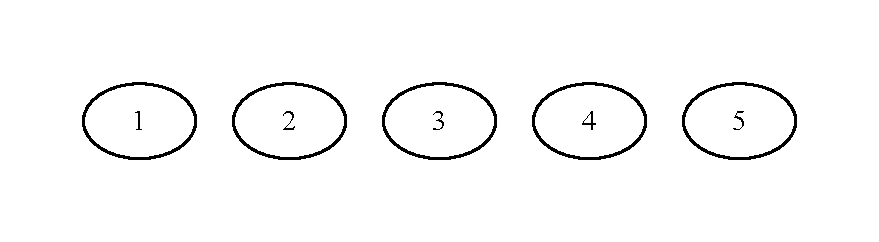
\includegraphics[width=0.6\textwidth]{images/randomgraph-01.pdf}
\caption{RandomGraph, stap 1}
\label{fig:randomgraph-01}
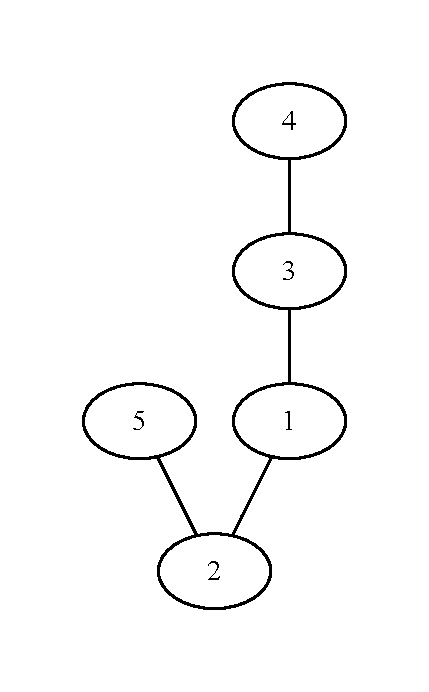
\includegraphics[width=0.3\textwidth]{images/randomgraph-02.pdf}
\caption{RandomGraph, stap 2}
\label{fig:randomgraph-02}
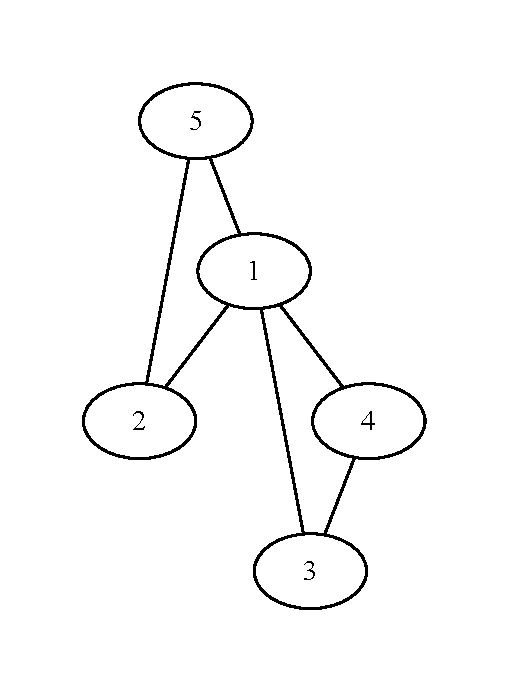
\includegraphics[width=0.3\textwidth]{images/randomgraph-03.pdf}
\caption{RandomGraph, stap 3}
\label{fig:randomgraph-03}
\end{center}
\end{figure}

\section{Output: Graphviz}
Het is handig als we grafen kunnen visualiseren, om de correctheid van bepaalde
delen van ons algoritme te testen. Daarom besliste ik een klasse
\verb#GraphDotWriter# te schrijven, deze bevindt zich in het package
\verb#graphviz# (in de map \verb#tests#). Deze klasse bevat functionaliteit om
grafen van de klasse \verb#Graph# uit te schrijven naar dot-bestanden. De
specificatie van deze dot-bestanden is te vinden op \verb#www.graphviz.org#.
Omdat we enkel simpele grafen willen outputten, is deze klasse niet zo complex.

\section{Het na\"ieve algoritme}

\subsection{Lazy genereren van embeddingen}
Ons na\"ieve algoritme overloopt alle embeddingen. Het is echter belangrijk dat
we de embeddingen op een \emph{lazy} manier genereren. Indien we de permutaties
\emph{strict} zouden genereren, zouden we een algoritme krijgen dat (weliswaar
met branching) het volgende idee implementeerd:

\lstset{language=Python}
\begin{lstlisting}
genus = +Infinity
for e in getEmbeddings(graph):
    eGenus = getGenus(e)
    if eGenus < genus:
        genus = eGenus
\end{lstlisting}

Hierbij is het probleem dat we pas informatie over het genus krijgen op het
moment dat e gegenereerd is. Als we hierop bounding criteria willen toepassen,
zouden we enkel de bladeren in onze zoekboom kunnen schrappen. Omdat we meer
willen schrappen, zoeken we dus naar een beter algoritme, waarin we vroeger
informatie over het genus verkrijgen.
\newline

\subsection{findGenus en findFaces}
Het genus van een graaf en een embedding $i$ wordt gegeven door
$v + f_i - e = 2 - 2g_i$. We weten $v$ en $e$ vast liggen, en enkel $f$ vari\"eert
als voor een graaf de embeddingen aflopen. Het zoeken van $min(g)$ komt dus
neer op het zoeken van $max(f)$, want
\begin{equation*}
min(g) = 1 - \frac{v + max(f) - e}{2}
\end{equation*}

\subsection{Algoritme: Het zoeken van het maximaal aantal vlakken}
Eerst zetten we de graaf die we krijgen als input om in een gerichte graaf. We
beginnen met een willekeurige (gerichte) boog $e_1$ die nog niet in een pad
ligt.  Stel dat op het einde van deze boog de top $v$ ligt. We nemen nu de
verzameling kandidaat bogen $E_v$ die op $e_i$ kunnen volgen. Deze stap is niet
triviaal en wordt verder beschreven in \ref{kandidaatbogen}. Nu moeten we branchen
voor elk element van $E_v$. We voegen de gekozen boog $e_{i+1}$ toe aan ons pad.
Indien deze boog dezelfde boog is als de eerste boog in ons pad, $e_1$, Hebben
we van ons pad een cykel gemaakt. Op dat moment kijken we of er nog bogen zijn
die niet in een pad liggen. Als dit het geval is, beginnen we een nieuw pad met
een willeukerige boog. Anders hebben we een volledige embedding gevonden, en
bevinden we ons in een blad van de zoekboom.
\newline

In de vorige paragraaf schreven we dat we als we op een gegeven moment een boog
toevoegen die dezelfde is als de eerste boog in ons voorlopige cykel, dat we
dan een vlak hebben. Maar we kunnen zelfs nog vroeger stoppen met een cykel,
namelijk \emph{op het moment dat we in de eerste top van de cykel terugkomen,
en we kunnen de cykel sluiten zonder dat dit de permutaties verstoord}.
\newline

Stel immers dat we in onze begintop komen en we kunnen de cykel sluiten. Als
we op dit moment branchen, zullen we na een bepaalde tijd weer terugkomen in
deze begintop, immers, de cykel moet gesloten worden. We krijgen dan een
cykel zoals in Figuur \ref{fig:octo} (met 1 onze begintop). We zien dat we
deze cykel eigenlijk kunnen splitsen in twee cykels (tenminste twee in het
algemene geval)! Aangezien we een embedding zoeken met zoveel mogelijk cykels,
is het dus niet verstanding om nog te branchen als we onze cykel kunnen sluiten.
Vandaar dat we dit niet doen.

\begin{figure}
\begin{center}
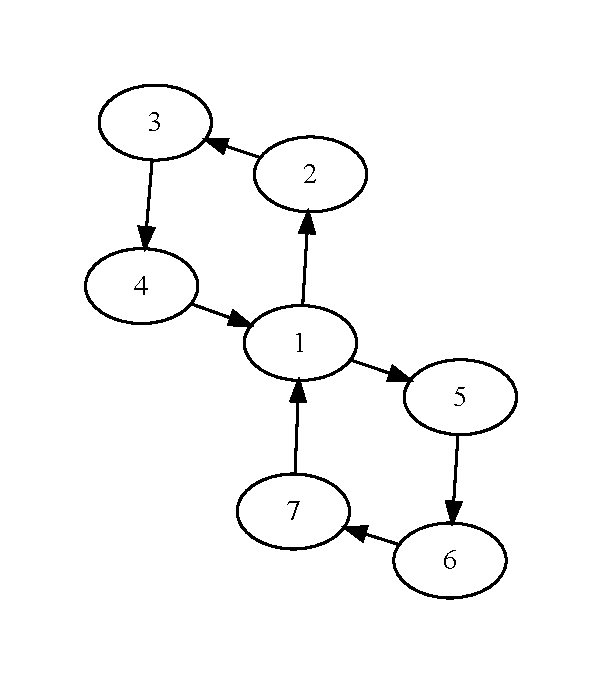
\includegraphics[width=0.6\textwidth]{images/octo.pdf}
\caption{Een cykel die gesplitst kan worden}
\label{fig:octo}
\end{center}
\end{figure}

\subsection{Het nemen van kadidaatbogen volgend op een boog}
\label{kandidaatbogen}
Onze embedding defini\"eert voor elke top een bepaalde volgorde van de bogen in
deze top. We slaan deze volgordes op in de klasse \verb#CycleNode#. Initieel kan
elke boog volgen op elke andere boog. We stellen dit voor als $n$ deelvolgordes
\begin{equation*}
(e_1) (e_2) (e_3) \dots (e_n)
\end{equation*}
voor een top met $n$ bogen. Stel dat we op een bepaald moment in ons algoritme
in de top toekomen via $e_i$ en weggaan via $e_j$. Vanaf dit moment moeten we
hiermee rekening houden, mochten we nog eens in de top komen. We slaan dit op
als
\begin{equation*}
(e_1) (e_2) (e_3) \dots (e_i e_j) \dots (e_n)
\end{equation*}
Hoe vinden we nu de kandidaatbogen? Stel dat we uit $e_i$ komen. We hebben in
onze top de volgende volgordes opgeslaan:
\begin{equation*}
(e_{a1} e_{a2} \dots e_{ax}) (e_{b1} e_{b2} \dots e_{by}) \dots (e_{c1} e_{c2} \dots e_{cz})
\end{equation*}
We weten dat er nog geen boog volgt op $e_i$, dus zal $e_i$ het laatste element
zijn in een deelvolgorde.
\newline

We kunnen bijvoorbeeld niet $e_{a2}$ als volgende boog kiezen, omdat we al
gedefini\"eerd hebben dat deze op $e_{a1}$ volgt. Stel dat $e_i = e_{ax}$,
dan kunnen we niet als volgende boog $e_{a1}$ kiezen, want op dat moment zouden
we de deelvolgorde \emph{sluiten}. Dit mag niet, want, zoals in de opgave
beschreven wordt, moeten we uiteindelijk een volgorde als $(e_1 e_2 \dots e_n)$
uitkomen, zodat als we de volgorde doorlopen, elke $e$ tegenkomen.
\newline

Meer algemeen zijn de deelkandidaten die kunnen volgen op $e_i$ alle $e_j$ die
voldoen aan twee voorwaarden:
\begin{itemize}
\item $e_j$ is het eerste element van een deelvolgorde
$(e_j e_{j+1} ... e_{j+n})$.
\item $e_j$ zit niet in dezelfde deelvolgorde als $e_i$.
\end{itemize}

Een uitzondering bestaat wanneer we slechts \'e\'en deelvolgorde 
$(e_1 e_2 \dots e_i)$ ($e_i$ is dan het laatste element, aangezien het als
enige $e$ nog geen opvolger heeft) meer hebben. Dit geval is echter triviaal,
dan is de enige kandidaat $e_1$.

\section{Bounding Criteria}

\subsection{Een ondergrens voor het maximaal aantal vlakken}
\label{ondergrens-maximaal-aantal-vlakken}
We kunnen bounden als we een ondergrens $m$ hebben voor het maximaal aantal
vlakken $F$. We zoeken immers $F$. Stel dat we in het algoritme zitten en we
hebben momenteel $f$ vlakken. We hebben eerder al een embedding gevonden met
$m$ vlakken. Stel dat we weten dat we $x$ vlakken kunnen maken met de bogen die
we op dat moment nog niet gebruikt hebben. Dat betekent dat we kunnen stoppen
met ons algoritme zodra
\begin{equation*}
f + x \leq m
\end{equation*}
want we weten dat
\begin{equation*}
m \leq F
\end{equation*}
en dus
\begin{equation*}
f + x \leq F
\end{equation*}
Dit laatste impliceert dat we toch geen embedding met meer vlakken zullen vinden
in de huidige branch van de zoekruimte, en dus kunnen we maar beter stoppen.
\newline

Het is nu de vraag hoe we $x$ kiezen. Om ons algoritme performant te maken,
willen we veel bounden, en dus willen we dat $f + x < m$ zoveel mogelijk
voorkomt. We willen $x$ dus zo klein mogelijk, maar natuurlijk nog altijd
correct, omdat we niet te vroeg willen bounden. We willen natuurlijk ook niet
te veel tijd besteden aan $x$ te berekenen, omdat zo het voordeel dat we krijgen
door bounding weer zal wegvallen.

\subsection{Pariteit van het aantal vlakken}
Als we de formule
\begin{equation*}
g = 1 - \frac{v + f - e}{2}
\end{equation*}
bekijken, en we weten dat $g$ altijd een geheel getal is, kunnen we hieruit
afleiden dat $v + f - e$ altijd even is. Dit betekend dat, aangezien $v$ en $e$
vastliggen voor de graaf, $f$ dezelfde pariteit zal behouden. Met andere
woorden, vinden we een embedding $E_1$ met $f_1$ vlakken, en een embedding $E_2$
met $f_2$ vlakken, dan weten we dat ofwel $f_1$ en $f_2$ beide even zijn, ofwel
beide oneven.

Als we ons boundingcriteria uit \ref{ondergrens-maximaal-aantal-vlakken}
bekijken,
\begin{equation*}
f + x \leq m
\end{equation*}
kunnen we dit nog verbeteren. Stel immers dat er een embedding kan gevonden met
aantal vlakken $f_1$ zodat $f_1 > m$. Aangezien $m$ ook een aantal vlakken
gevonden in een embedding voorstelt, zal wegens het feit dat $f_i$ en $m$
dezelfde pariteit bezitten ook gelden dat $f_1 > m + 1$. We kunnen dus nog iets
sneller bounden, namelijk zodra
\begin{equation*}
f + x \leq m + 1
\end{equation*}

\subsection{Een eerste poging}
\label{een-eerste-poging}
We weten dat we om een vlak te maken tenminste 3 bogen nodig hebben. We
houden dus het aantal bogen dat we nog niet gebruikt hebben bij in $l$. We vinden
dan dat
\begin{equation*}
x = \lfloor\frac{max(2, c) + l}{3}\rfloor
\end{equation*}
met $c$ het aantal bogen in de huidige cykel. We tellen $max(2, c)$ op bij $l$
omdat we zo $x$ preciezer maken. Als we al meer dan 2 bogen in de huidige
cykel hebben, kunnen we met 1 boog uit $l$ een extra cykel maken. Anders
hebben we er $3 - c$ nodig. Dit zit op deze manier ook in onze berekening.

\subsection{Girth van een graaf}
In \ref{een-eerste-poging} gingen we ervan uit dat we tenminste 3 bogen nodig
hebben om een vlak te maken. Dit is natuurlijk altijd waar, maar stel dat we
een graaf hebben als in Figuur \ref{fig:cube}. Als we deze graaf bekijken, zien
we dat we tenminste 4 bogen nodig hebben om een vlak te maken. Aan de hand van
deze informatie kunnen we een betere $x$ opstellen voor deze graaf.
\begin{equation*}
x = \lfloor\frac{max(3, c) + l}{4}\rfloor
\end{equation*}
We vragen ons natuurlijk af hoe we dit algemeen kunnen toepassen. Het
\emph{girth} van een graaf is de lengte van kleinste cykel. Dit is precies wat
we nodig hebben! We kunnen dus voor elke graaf schrijven:
\begin{equation*}
x = \lfloor\frac{max(girth - 1, c) + l}{girth}\rfloor
\end{equation*}
Hoe moeten we het \emph{girth} van een graaf nu berekenen? We kiezen voor een
eenvoudige manier. We starten vanuit elke top van de graaf een
\emph{breadth-first search} en houden de diepte bij. Op het moment dat we een
top terechtkomen waar we al geweest zijn, hebben we de kleinste cykel van de
graaf gevonden waar de wortel van de BFS in ligt. Door een BFS te starten vanuit
elke top, kunnen we de kleinste cykel van de gehele graaf bepalen.  Dit
algoritme is ge\"implementeerd in de klasse \verb#FindGirth#.
\newline

In het slechtste geval moet de BFS voor elke top de gehele graaf doorzoeken. De
tijdscomplexiteit voor dit algoritme wordt dus naar boven begrensd door $O(ve)$
met $v$ het aantal vertices, en $e$ het aantal (ongerichte) bogen.

\begin{figure}
\begin{center}
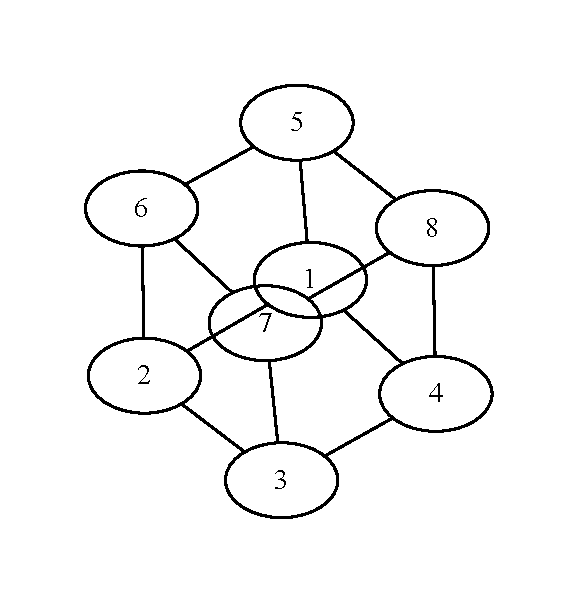
\includegraphics[width=0.4\textwidth]{images/cube.pdf}
\caption{Een graaf met \emph{girth} 4}
\label{fig:cube}
\end{center}
\end{figure}

\subsection{Nog een beetje beter}
Door de manier waarop \verb#DefaultGraph# ge\"implementeerd is, kunnen we
in constante tijd kijken of er een boog bestaat tussen twee toppen. Dit kunnen
we gebruiken om onze $x$ nog een beetje beter te maken.
\begin{equation*}
x = 1 + \lfloor\frac{l - n}{girth}\rfloor
\end{equation*}
met $l$ opnieuw het aantal bogen dat nog niet gebruikt is, en $n$ staat hier
voor het aantal bogen voor dat we nog nodig hebben om het huidige vlak af te
maken.
\newline

Het aantal vlakken dat we nog kunnen maken is dus 1 (namelijk, het vlak dat we
momenteel aan het maken zijn) plus $\lfloor\frac{l - n}{girth}\rfloor$:
het aantal bogen dat we nog over zullen hebben nadat het huidige vlak af is,
gedeeld door het \emph{girth} van de graaf.
\newline

Nu moeten we dus nog vinden wat $n$ is, dus het minimaal aantal bogen dat we
nog nodig hebben voor het huidige vlak af te maken. Stel $c$ het aantal bogen
dat we al gebruikt hebben in het huidige vlak. Als $c < girth$, dan
$n = girth - c$.
\newline

Anders, als $c \geq girth$, dan zijn er twee mogenlijkheden. Als de huidige top
een buur is van de top waar we het vlak begonnen zijn, dan $n = 1$. Anders
hebben we nog zeker 2 vlakken nodig, en dus $n = 2$.
\newline

\section{Heuristieken}

\subsection{Een smalle stam voor de zoekboom}
Intu\"itief willen we een zoekboom die een smalle stam heeft en een brede kruin
(zoals in Figuur \ref{fig:good-tree}), in plaats van een zoekboom met een brede
stam en een smalle kruin (zoals in Figuur \ref{fig:bad-tree}). Met andere
woorden, we willen dat ons algoritme in het begin zo weinig mogelijk moet
branchen, en naarmate we dieper in de zoekboom afdalen, mag het meer branchen.
\newline

Het voordeel hiervan is dat wanneer we delen van de zoekboom mogen uitschakelen,
meestal grotere delen kunnen uitschakelen.
\newline

\begin{figure}
\begin{center}
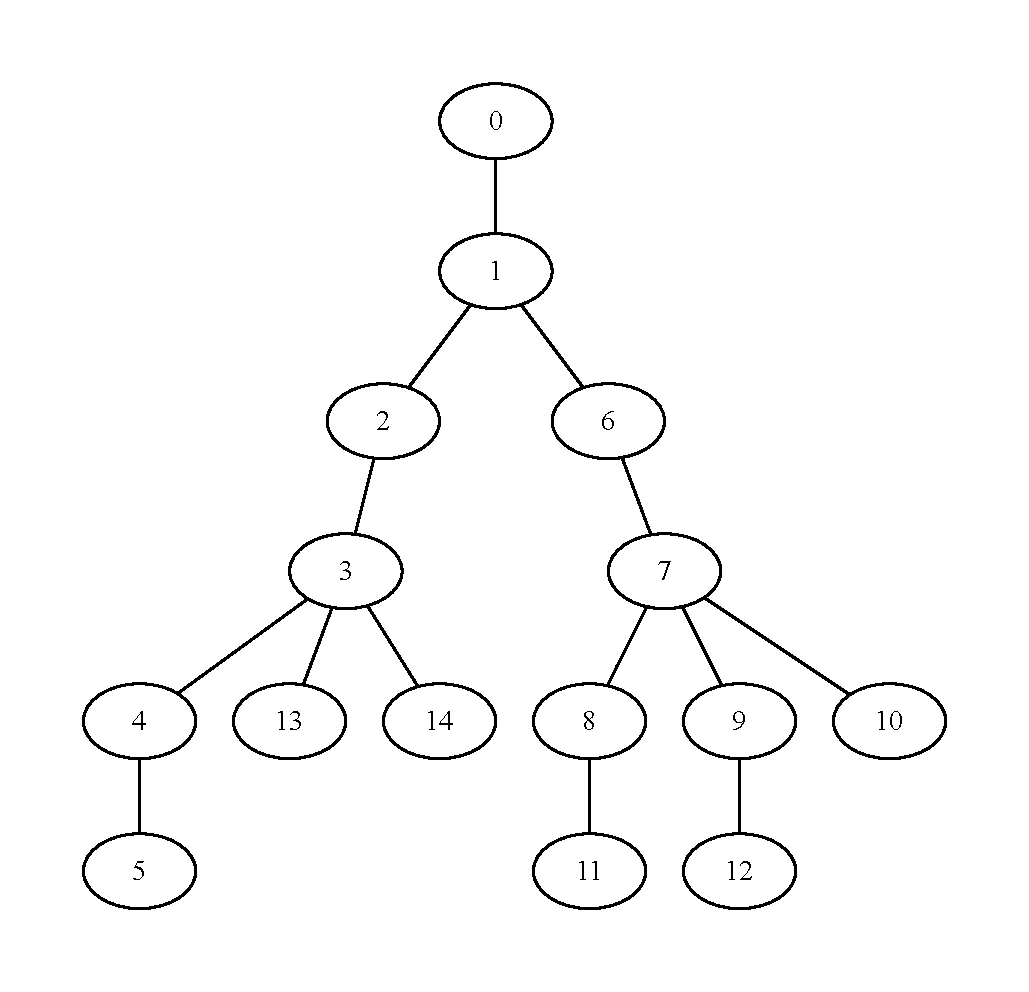
\includegraphics[width=0.6\textwidth]{images/good-tree.pdf}
\caption{Een boom met een smalle stam en een brede kruin}
\label{fig:good-tree}
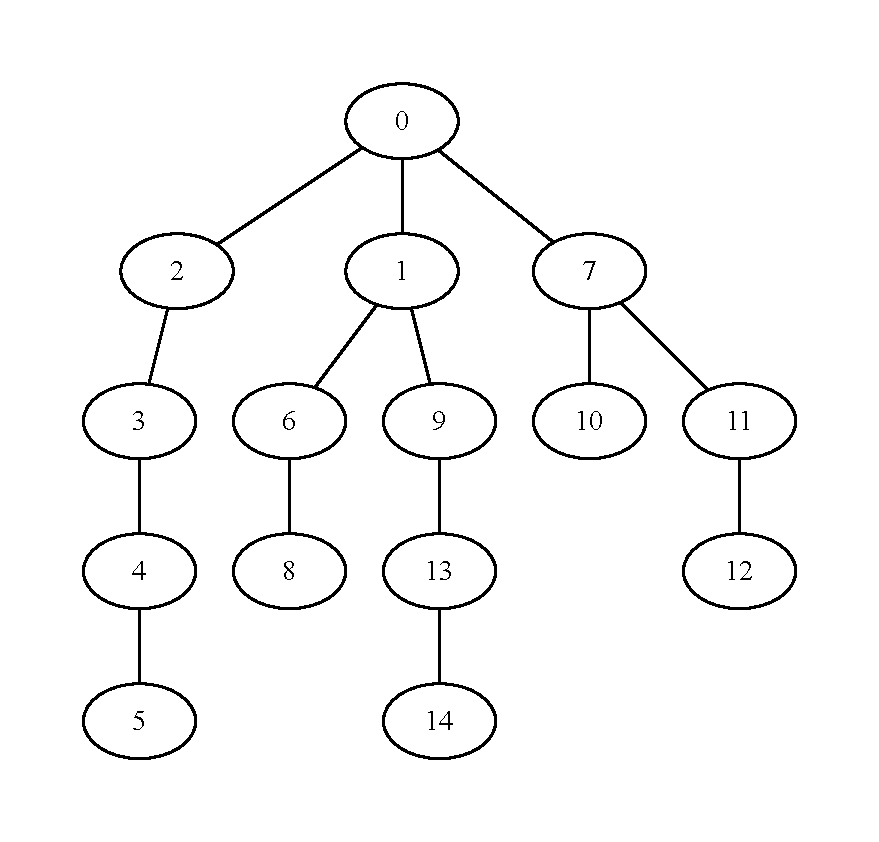
\includegraphics[width=0.6\textwidth]{images/bad-tree.pdf}
\caption{Een boom met een brede stam en een smalle kruin}
\label{fig:bad-tree}
\end{center}
\end{figure}

De vraag is natuurlijk hoe we onze zoekboom een zodanige vorm kunnen geven. Dit
is echter vrij eenvoudig. We weten dat ons algoritme zal branchen als we in een
top staan, en er zijn meerdere kandidaatbogen. Het aantal branches wordt
natuurlijk bepaald door het aantal kandidaatbogen. Het aantal kandidaatbogen is
dan weer grotendeels afhankelijk van het aantal bogen in die top.
\newline

We willen dus dat ons algoritme eerst de toppen bezoekt met weinig bogen, en
vervolgens de toppen met meer bogen. Dit implementeren we door de toppen van
de graaf te sorteren op het aantal bogen.
\newline

Verrassend genoeg vertraagd dit het algoritme enorm (zie Figuur 
\ref{fig:bounded-vs-sorted}). Dit is zeer
contra-intu\"itief en we willen natuurlijk een verklaring. We schrijven een
klasse \verb#ShowTreeFindGenus# als subklasse van \verb#FindGenus# met als
bedoeling de call tree van ons algoritme op een verstaanbare manier te
visualiseren. Hiertoe gebruikt het ook de \emph{DOT-taal} van graphviz.
\newline

\begin{figure}
\begin{center}
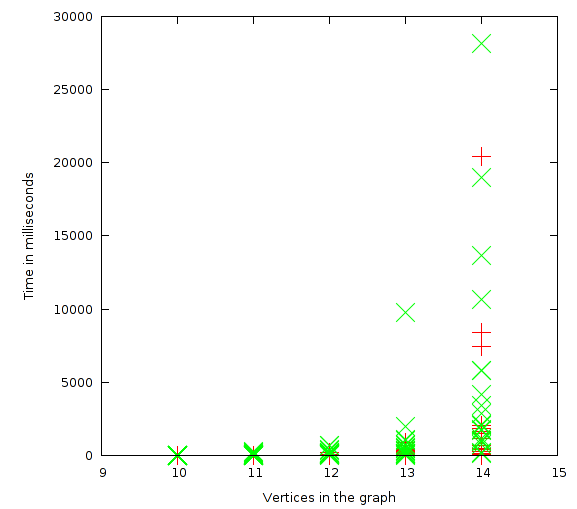
\includegraphics[width=\textwidth]{images/bounded-vs-sorted.png}
\caption{We zien dat de tijden van het algoritme met sorteren (groen) duidelijk
boven de tijden zonder sorteren (rood) liggen.}
\label{fig:bounded-vs-sorted}
\end{center}
\end{figure}

Aan het sorteren zelf kan het niet liggen, dit is een zeer snelle operatie
die slechts \'e\'enmaal gebeurt, namelijk bij het aanmaken van onze graaf.
We aanschouwen de call tree met sorteren (Figuur \ref{fig:sorted-call-tree})
en de call tree zonder sorteren (Figuur \ref{fig:default-call-tree}).
\newline

We zien onmiddelijk dat de call tree zonder sorteren veel eenvoudiger is!
Ook het aantal bladeren in de boom is verschillend. Dit verschil kan enkel
veroorzaakt worden door de eerste boog die we kiezen in een pad (immers, de
eerste boog kiezen we telkens willekeurig, voor de andere bogen proberen we
telkens alle mogenlijkheden). We zien ook dat de gesorteerde call tree
helemaal geen smalle stam en brede kruin heeft. We concluderen dat elke zoekboom
voor dit algoritme een relatief brede stam zal hebben, omdat er naar het einde
van ons algoritme toe sowieso minder mogenlijkheden overblijven (veel bogen
zijn al gekozen).
\newline

Het is dus soms beter om de eerste boog te kiezen in een top met relatief
veel bogen, zodat al tenminste \'e\'en boog daar gefixeerd is. Dit is
echter niet altijd geval, en hangt sterk af van de graaf in kwestie. We zullen
er dus voor kiezen om onze call tree niet te veranderen.

\begin{figure}
\begin{center}
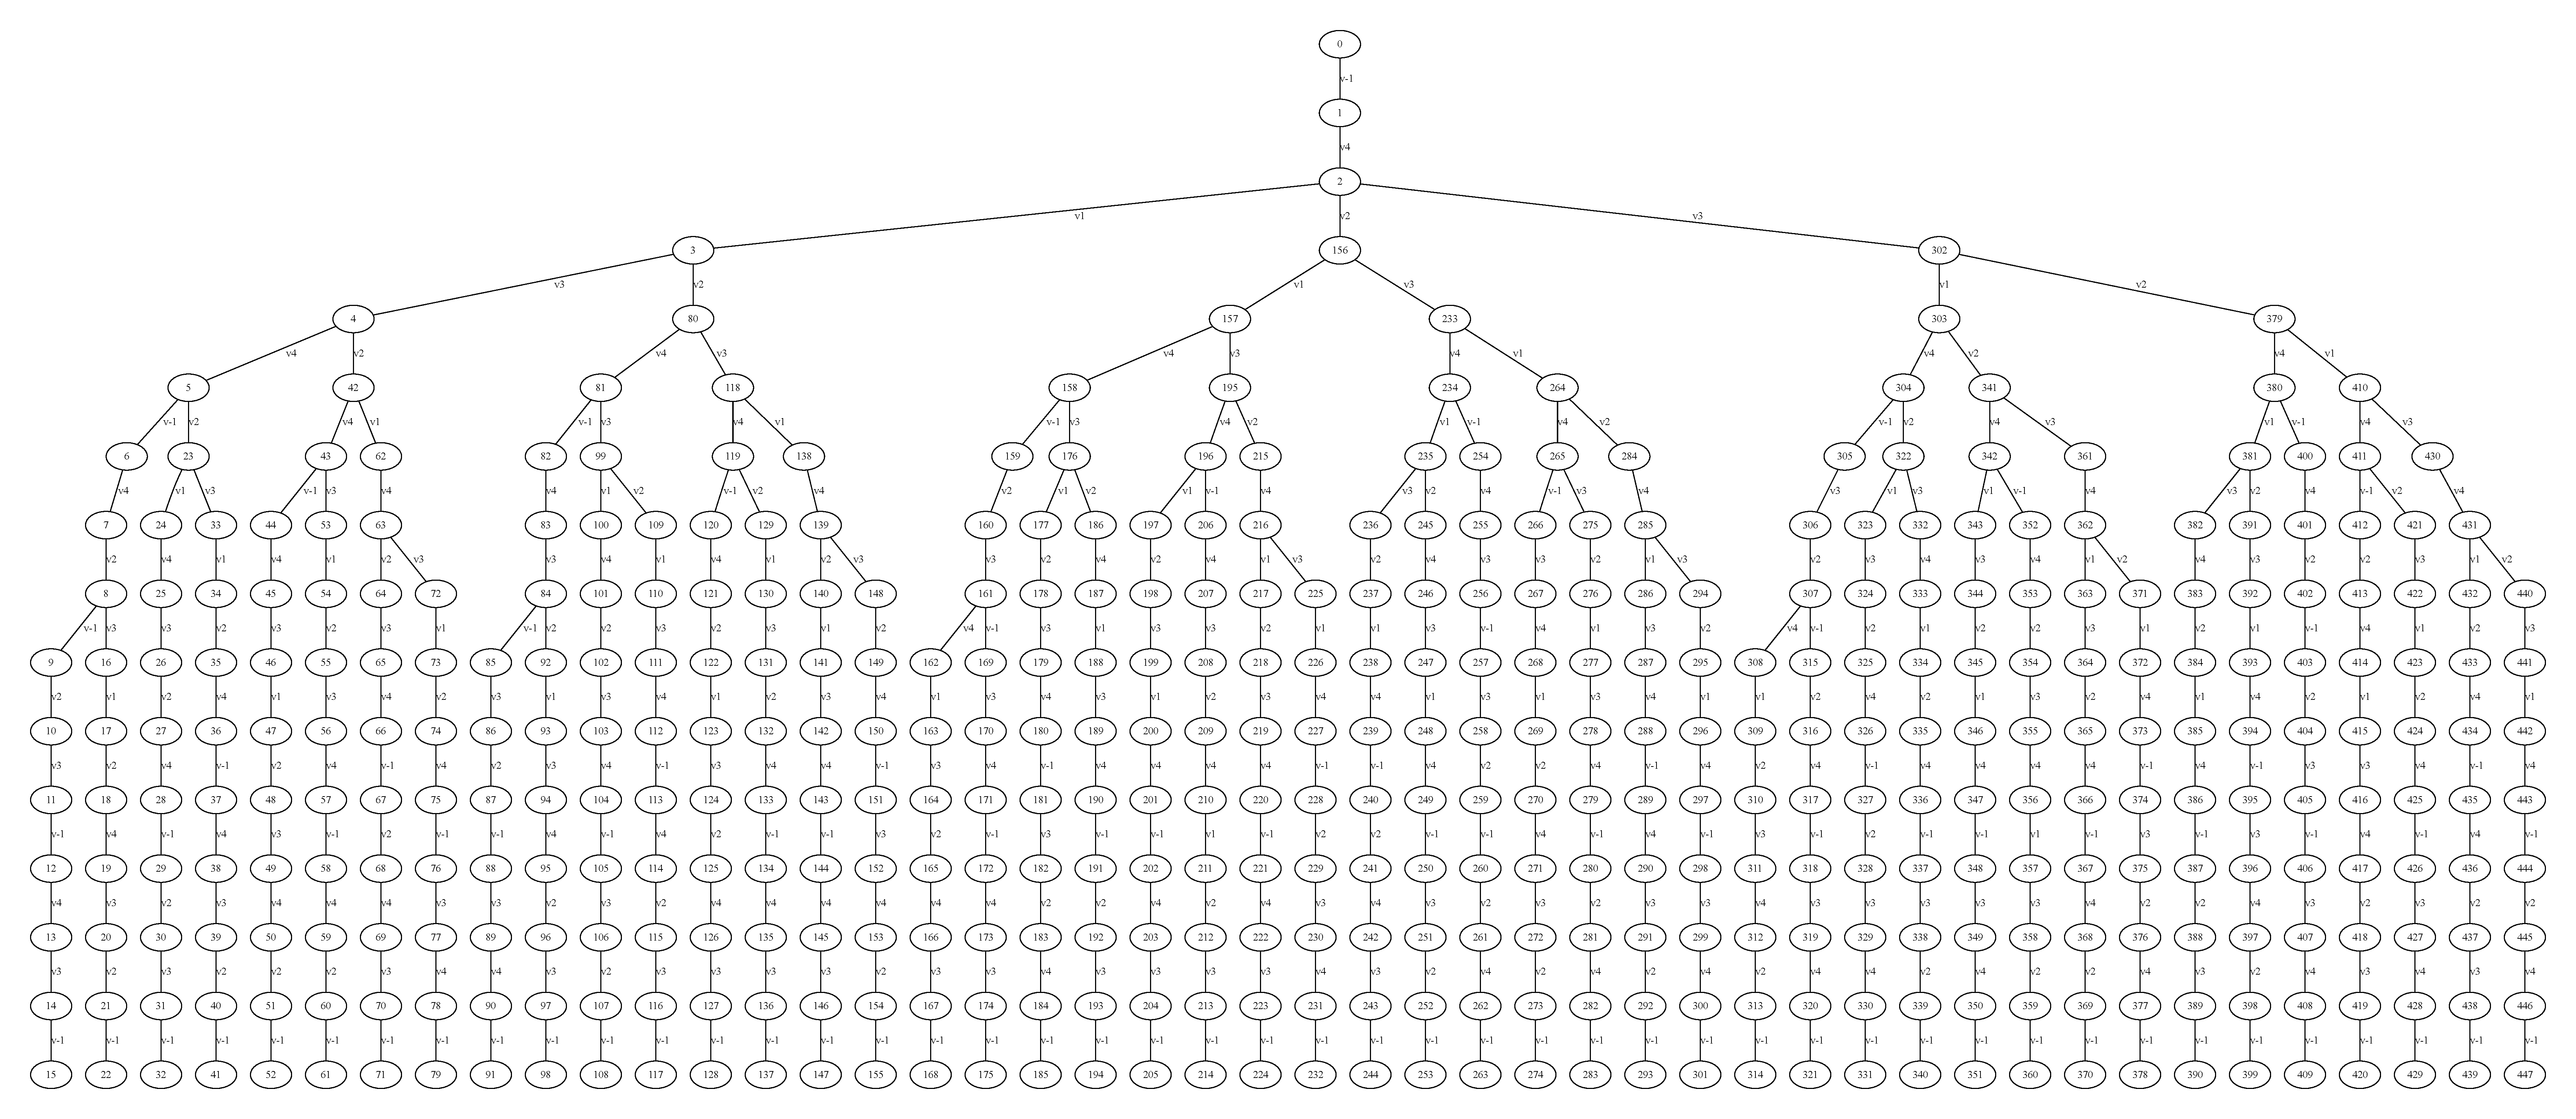
\includegraphics[width=\textwidth]{images/sorted-call-tree.pdf}
\caption{De call tree met sorteren}
\label{fig:sorted-call-tree}
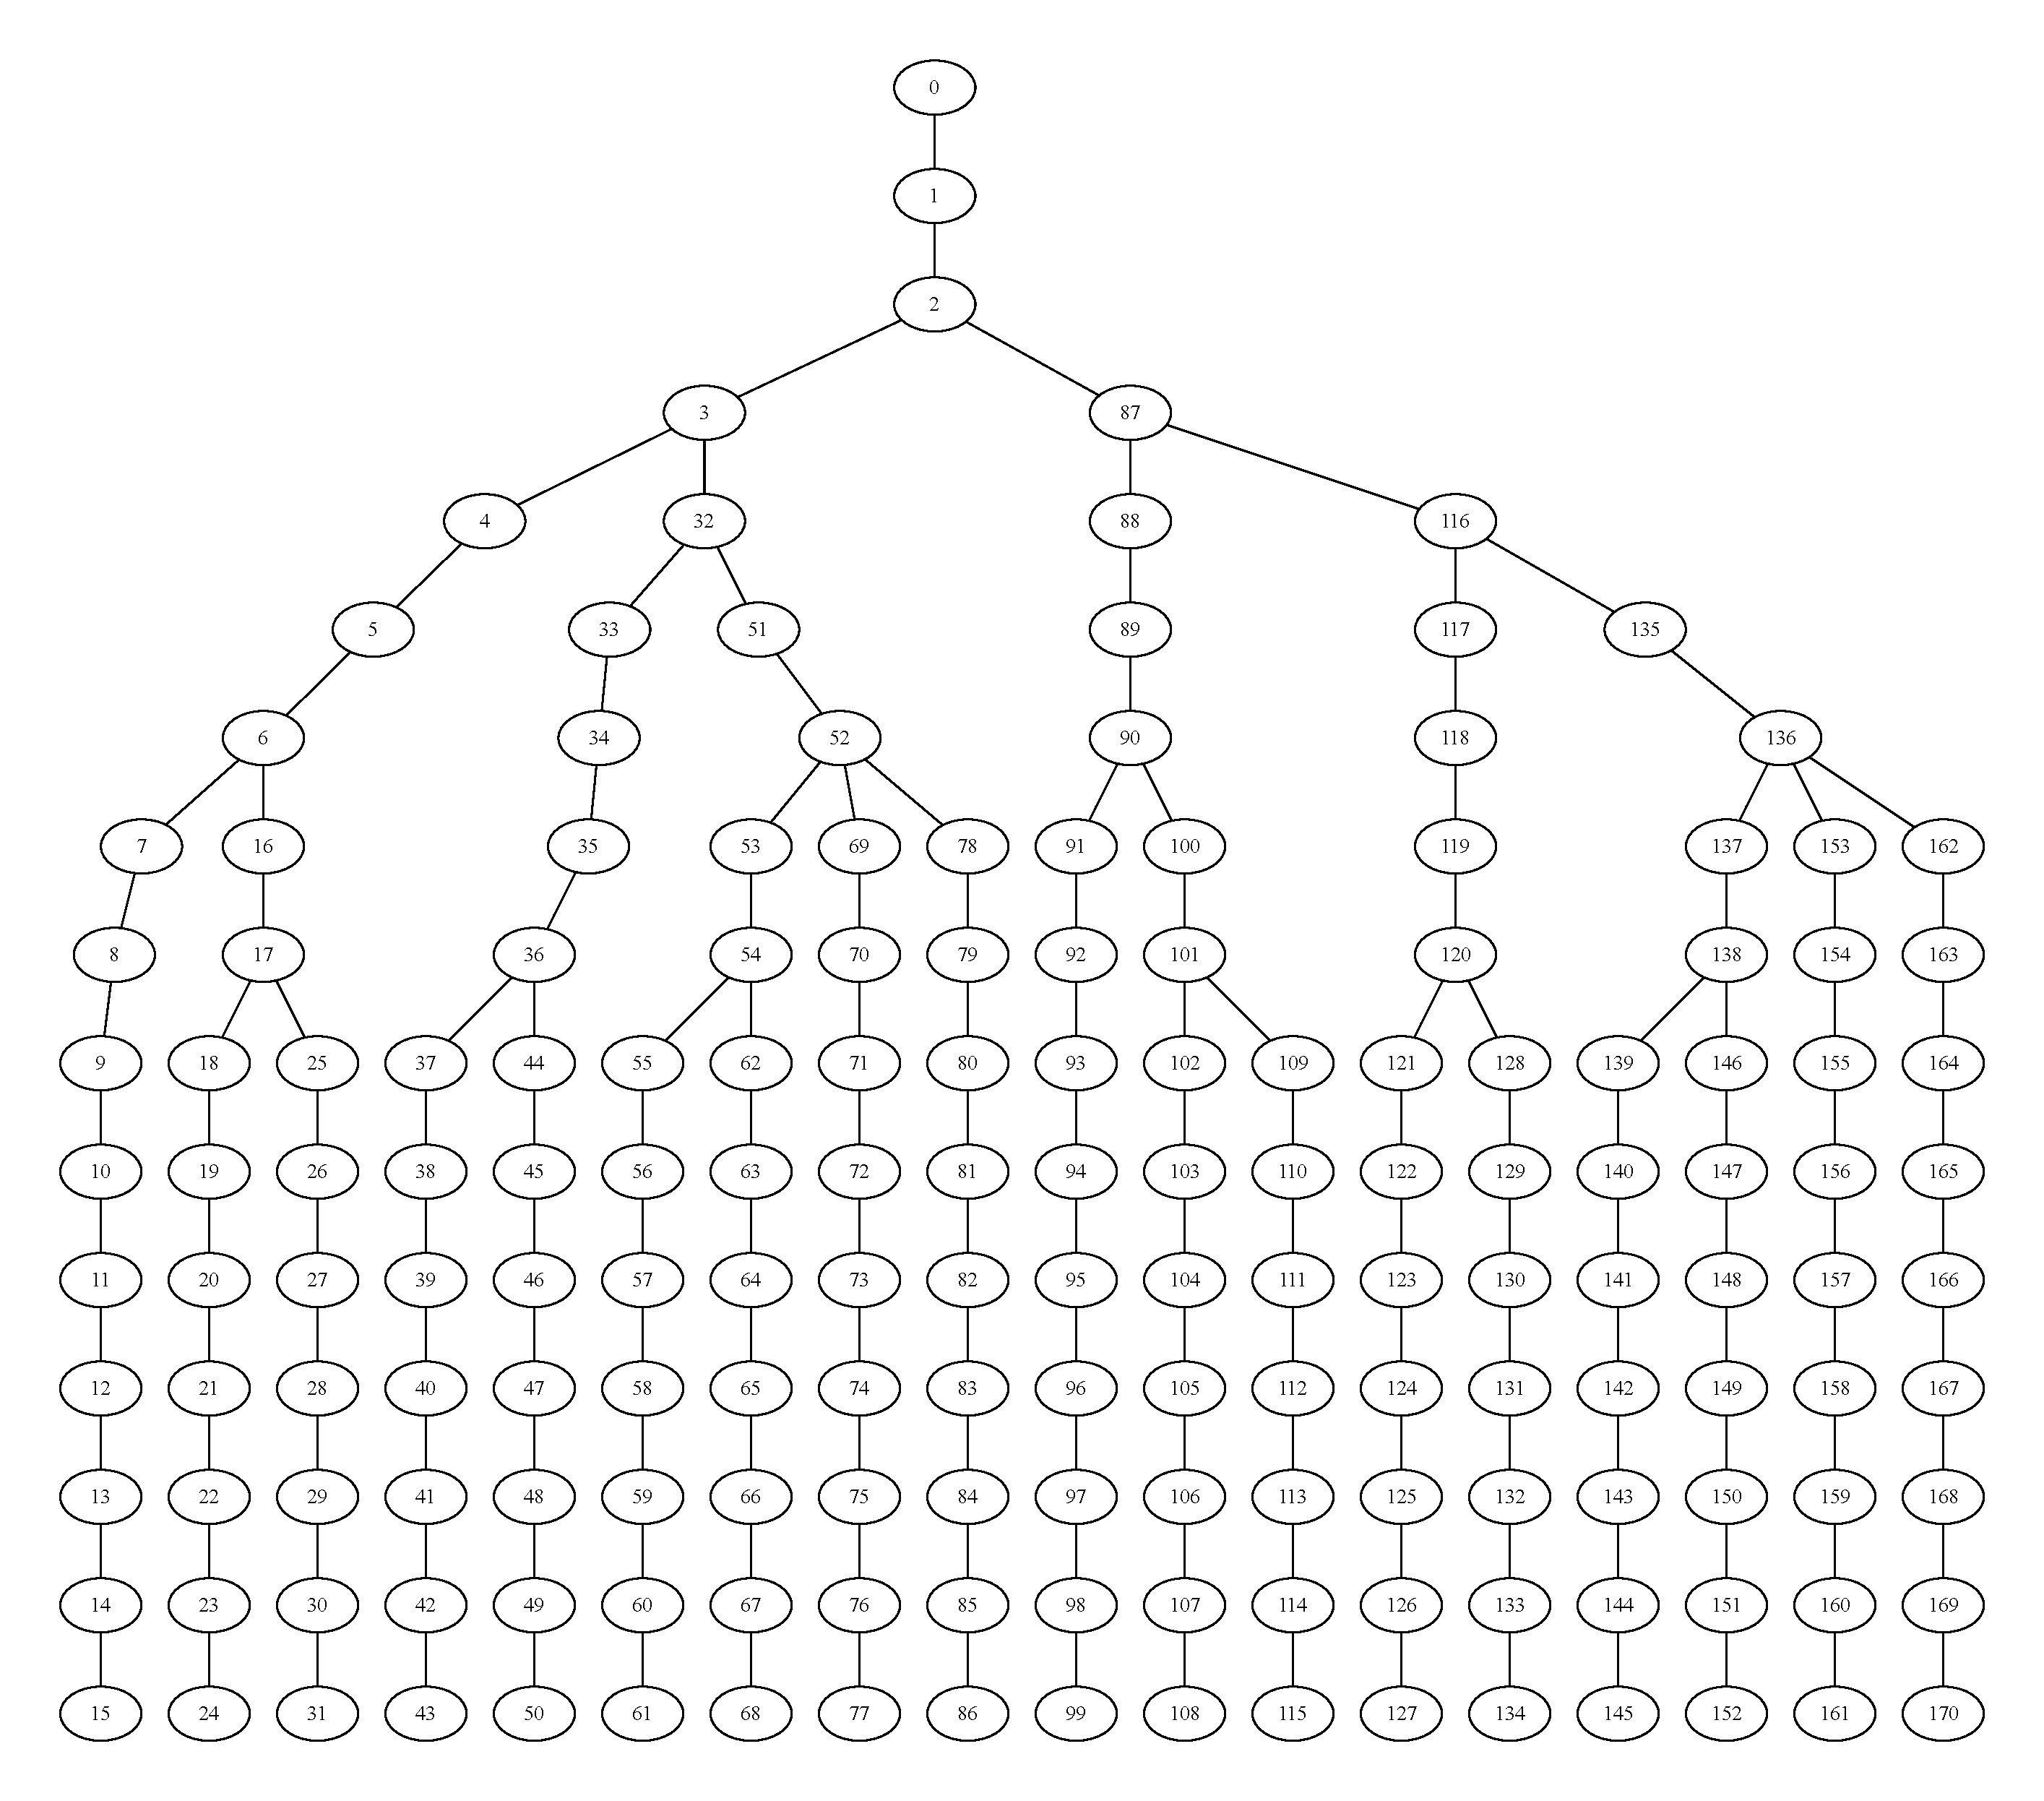
\includegraphics[width=\textwidth]{images/default-call-tree.pdf}
\caption{De call tree zonder sorteren}
\label{fig:default-call-tree}
\end{center}
\end{figure}

\end{document}
